%% template-chordsty.tex
%% Copyright 2024 Douglas Joziel Bitencourt Freitas
%
% This work may be distributed and/or modified under the
% conditions of the LaTeX Project Public License, either version 1.3
% of this license or (at your option) any later version.
% The latest version of this license is in
%   https://www.latex-project.org/lppl.txt
% and version 1.3c or later is part of all distributions of LaTeX
% version 2008 or later.
%
% This work has the LPPL maintenance status `maintained'.
% 
% The Current Maintainer of this work is Douglas Joziel Bitencourt Freitas.
%
% This work consists of the files template-chordsty.tex and qrcode.tex,
% and the derived file chordsty.sty.

\documentclass[
    a4paper,
    12pt
]{article}

% Pacotes
\usepackage[
    fontepadrao=fourier,
    corcifra=FF4500,
    esquerda=2.5cm,
    direita=2.5cm,
    superior=2.5cm,
    inferior=2.5cm,
    logomarca=true,
    numerotrastes=4
]{chordsty}

% Informações
\titulo{GRANDE É O SENHOR}
\artista{Eli Soares}

% Extras
\linkmusica{https://www.youtube.com/watch?v=oaedoTm7xpQ}
\referencias{
    Sl 48.1--2\\
    1Co 15.57\\
    Sl 95.6\\
    Jr 31.3\\
    Is 40.28
}
\palavraschave{
    Louvor\\
    Poder\\
    Confiança\\
    Gratidão\\
    Devoção
}

% Documento
\begin{document}

% QR-Code, referências e palavras-chave
\extras

% Cifra
\begin{songs}{}
    \beginsong{\showtitulo}[by={\showartista}]
    
    \transpose{0}
    %\preferflats
    %\prefersharps
    
    \meter{4}{4}
    \beginverse
    \parte{INTRODUÇÃO} \esp \obs[2]{\musQuarter~= 60 \esp\itshape Com melodia de \caixa{FRASE}}
    \barra \esp \[C\fns{7M}] \esp \[G\bxo{B}] \esp \barra \esp \[A\fns{m7}] \esp \[G\bxo{B}] \esp \barra \esp \[C\fns{7M}] \esp \[G\bxo{B}] \esp \barra \esp \[A\fns{m7}] \esp \barradupla \esp \obs{\itshape Dim. \dinamica{p}}
    %\hspace*{0.235em}\barra
    \endverse
    
    \beginverse
    \parte{A} \esp \obs[2]{\itshape Vocal unis.}
    \[G\fns{(add9)}]Grande é o Se\[C\bxo{G}]nhor e mui digno de lou\[G\fns{(add9)}]vor
    Na ci\[C\bxo{G}]dade do nosso Deus, Seu \[D\bxo{G}]santo \[E\fns{m7}]monte \[D\bxo{F\ss}]
    \[G\fns{(add9)}]Alegria de toda \[A\fns{m7}]ter\[B\fns{m7}]ra \esp \[C\fns{7M}] \esp \[D\fns{4}] \esp \barradupla \esp \obs{Cresc. \dinamica{mf}}
    \endverse
    
    \beginverse
    \parte{B} \esp \obs[2]{\itshape Vocal unis.}
    \[G\fns{(add9)}]Grande é o Se\[C\bxo{G}]nhor em quem nós temos a vi\[G\fns{(add9)}]tória
    E que \[C\bxo{G}]nos ajuda contra o \[D\bxo{G}]ini\[E\fns{m7}]migo \[D\bxo{F\ss}]
    Por \[G\fns{(add9)}]isso diante dEle nos pros\[A\fns{m7}]tra\[B\fns{m7}]mos \esp \[C\fns{7M}] \esp \[D\fns{4}] \esp \barradupla \esp \obs{Cresc. \dinamica{f}}
    \endverse
    
    \beginchorus
    \tab \parte{REFRÃO} \esp \obs[2]{\itshape Div. vocal}
    \tab Que\[G\fns{(add9)}]remos o teu nome engrande\[D\bxo{G}]cer 
    \tab \[C\fns{7M}]E agradecer-\[G\bxo{B}]Te por Tua \[A\fns{m7}]obra em nossas \[D\fns{4}]vidas
    \tab Con\[G\fns{(add9)}]fiamos em Teu infinito a\[D\bxo{G}]mor,
    \tab Pois \[C\fns{7M}]só Tu és o Deus eter\[G\bxo{B}]no \esp \obs{Síncope}
    \tab \[A\fns{m7}]Sobre toda \[D\fns{4}]terra e céu \esp \barradupla \esp \obs{Tético ao \caixa{INTERLÚDIO}}
    \endchorus
    
    \beginverse
    \parte{INTERLÚDIO} \esp \obs[2]{\itshape Com melodia de \caixa{FRASE}}
    \barra \esp \[C\fns{7M}] \esp \[G\bxo{B}] \esp \barra \esp \[A\fns{m7}] \esp \[G\bxo{B}] \esp \barra \esp \[C\fns{7M}] \esp \[G\bxo{B}] \esp \barra \esp \[A\fns{m7}] \esp \[G\bxo{B}] \esp \barradupla \esp \obs{\itshape Dim. \dinamica{mf}}
    %\hspace*{0.235em}\barra
    \endverse
    
    \beginverse
    \parte{C} \esp \obs[2]{\itshape Vocal unis.}
    \[G\fns{(add9)}]Grande é o Se\[C\bxo{G}]nhor em quem nós temos a vi\[G\fns{(add9)}]tória
    E que \[C\bxo{G}]nos ajuda contra o \[D\bxo{G}]ini\[E\fns{m7}]migo \[D\bxo{F\ss}]
    Por \[G\fns{(add9)}]isso diante dEle nos pros\[A\fns{m7}]tra\[B\fns{m7}]mos \esp \[C\fns{7M}] \esp \[D\fns{4}] \esp \barradupla \esp \obs{Cresc. \dinamica{f}}
    \endverse
    
    \beginchorus
    \tab \parte{REFRÃO} \esp \obs[2]{\itshape Div. vocal}
    \tab Que\[G\fns{(add9)}]remos o teu nome engrande\[D\bxo{G}]cer 
    \tab \[C\fns{7M}]E agradecer-\[G\bxo{B}]Te por Tua \[A\fns{m7}]obra em nossas \[D\fns{4}]vidas
    \tab Con\[G\fns{(add9)}]fiamos em Teu infinito a\[D\bxo{G}]mor,
    \tab Pois \[C\fns{7M}]só Tu és o Deus eter\[G\bxo{B}]no \esp \obs{Síncope}
    \tab \[A\fns{m7}]Sobre toda \[D\fns{4}]terra e céu \esp \barradupla \esp \obs{Segue base e vocal (sem ritmo) \esp $\mid$ \esp Dim. \dinamica{mf}}
    \tab Que\[G\fns{(add9)}]remos o teu nome engrande\[D\bxo{G}]cer 
    \tab \[C\fns{7M}]E agradecer-\[G\bxo{B}]Te por Tua \[A\fns{m7}]obra em nossas \[D\fns{4}]vidas
    \tab Con\[G\fns{(add9)}]fiamos em Teu infinito a\[D\bxo{G}]mor,
    \tab Pois \[C\fns{7M}]só Tu és o Deus eter\[G\bxo{B}]no \esp \obs{Síncope}
    \tab \[A\fns{m7}]Sobre toda \[D\fns{4}]terra e \[G\fns{(add9)}]céu \esp \barrafinal \esp \obs{\caixa{FIM}}
    \endchorus
    
    % Material de apoio
    \vfill
    \beginverse
    \parte{FRASE}
    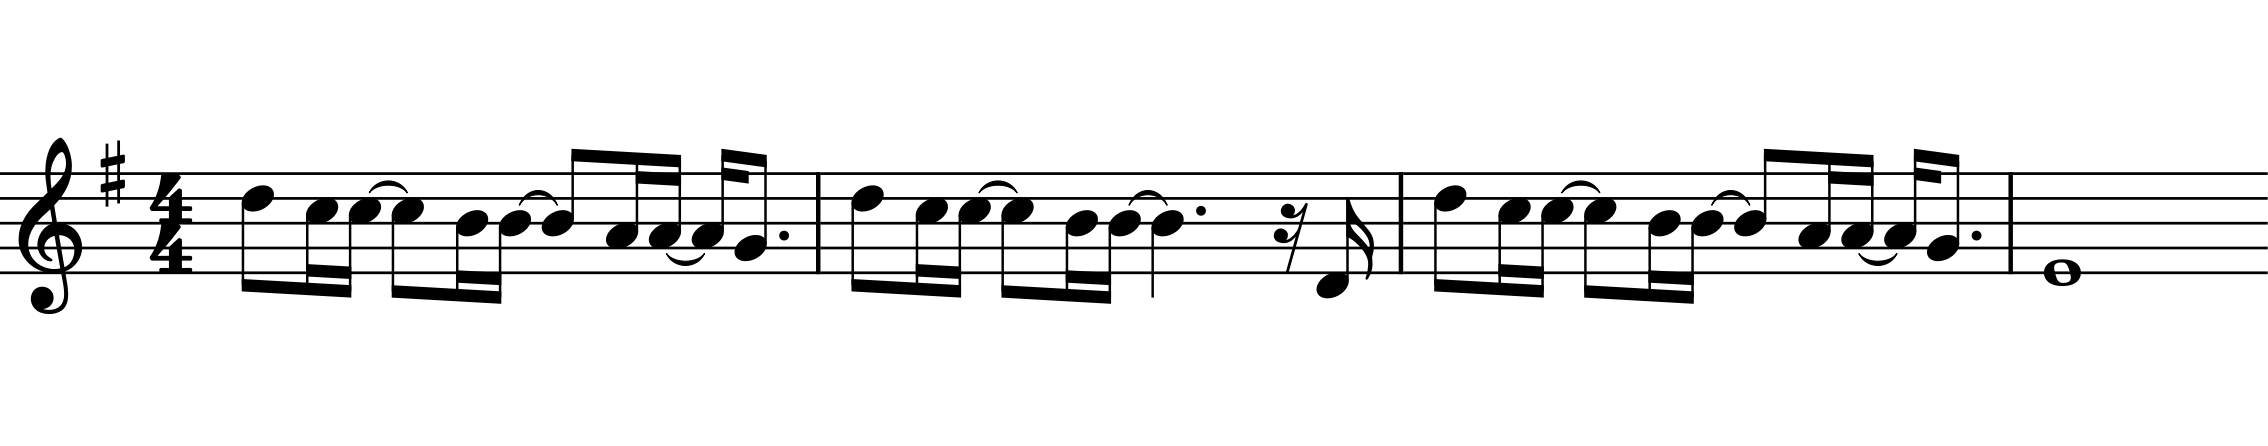
\includegraphics[trim={0 0.3in 0 0.3in}, clip]{frase}
    \endverse
    
    \beginverse
    \parte{RITMO}
    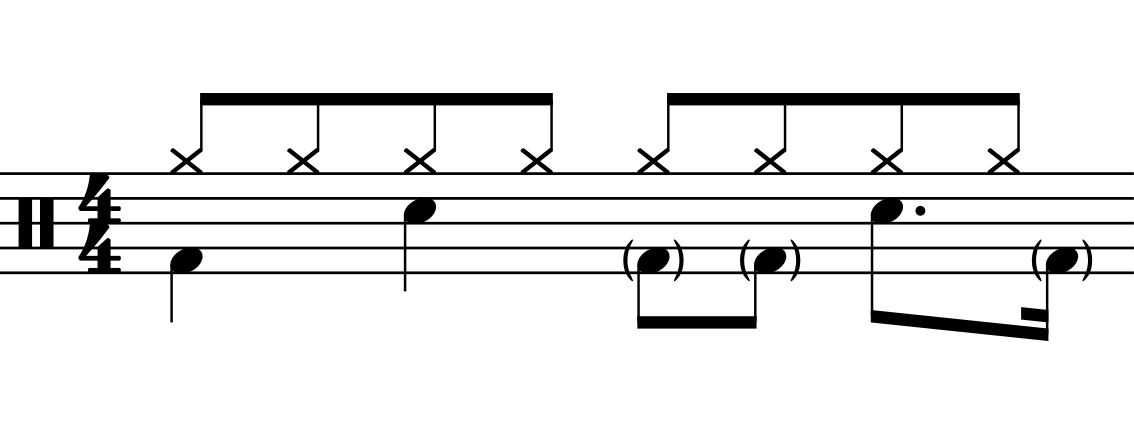
\includegraphics[trim={0 0.2in 0 0.05in}, clip]{ritmo}
    \endverse
    
    \newpage
    \beginverse
    \parte{DICIONÁRIO DE ACORDES}
    {\centering
        \begin{tabular}{ccccc}
            \acorde{C\fns{7M}}{-1,3,2,0,0,0}{X,C,E,G,B,E}{0}{}{} &
            \acorde{G\bxo{B}}{-1,2,0,0,3,3}{X,B,D,G,D,G}{0}{}{} &
            \acorde{A\fns{m7}}{-1,0,2,0,1,0}{X,A,E,G,C,E}{0}{}{} &
            \acorde{G\fns{(add9)}}{3,-1,0,2,3,3}{G,X,D,A,D,G}{0}{}{} &
            \acorde{C\bxo{G}}{3,-1,2,0,1,3}{G,X,E,G,C,G}{0}{}{} \\
            \acorde{D\bxo{G}}{3,-1,0,2,3,2}{G,X,D,A,D,F\ss}{0}{}{} &
            \acorde{E\fns{m7}}{0,2,2,0,3,3}{E,B,E,G,D,G}{0}{}{} &
            \acorde{D\bxo{F\ss}}{2,0,0,2,3,2}{F\ss,A,D,A,D,F\ss}{0}{}{} &
            \acorde{B\fns{m7}}{-1,2,4,2,3,2}{X,B,F\ss,A,D,F\ss}{2}{5}{} &
            \acorde{D\fns{4}}{-1,-1,0,2,3,3}{X,X,D,A,D,G}{0}{}{} 
        \end{tabular}
    }
    \endverse
    
    \endsong
\end{songs}

\end{document}
